

\section{Extensible Queries and Transformations}
\label{SECT:extensible}

\begin{figure}
  \centering

  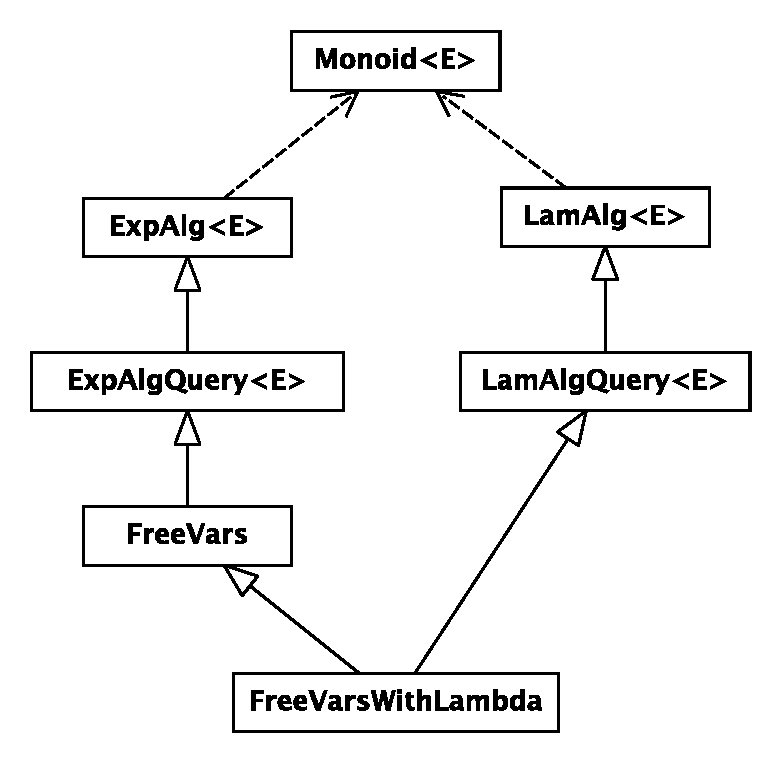
\includegraphics[width=0.45\linewidth]{extendQuery}
  \hspace*{2pt}
  \vline
  \hspace*{2pt}
  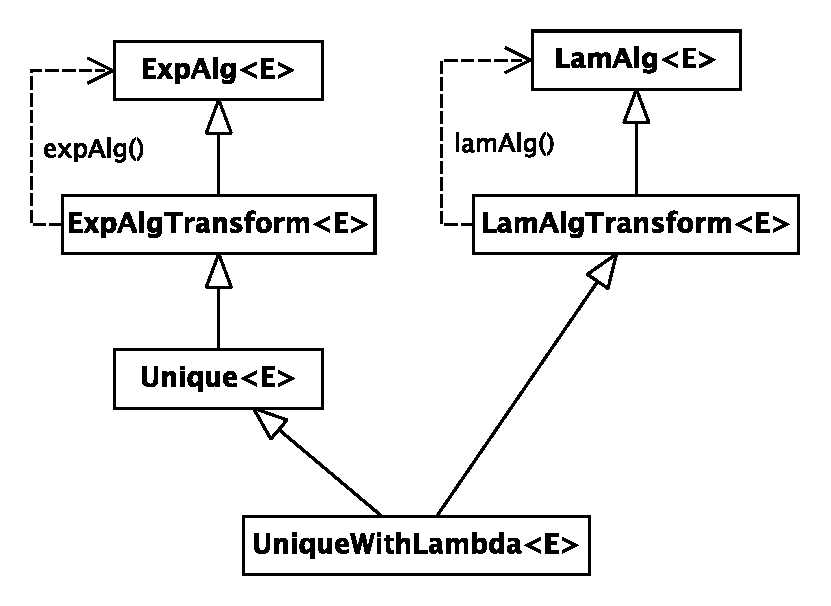
\includegraphics[width=0.45\linewidth]{extendTransform}
  
  \caption{Extension of the \texttt{FreeVars} query (left) and the \texttt{Unique} transformation}
  \label{FIG:extension}
\end{figure}

\noindent \name queries and transformation inherit  modular extensibility from the Object Algebra design pattern.
New transformations or queries are simply added by extending the interfaces generated by \name.
More interestingly, however, it is also possible to extend the data type with new constructors.
Here we briefly describe how queries and transformations can be extended in this case.
Figure~\ref{FIG:extension} gives a high level overview of the approach.


Consider the extension of the expression language with a lambda and application constructs.
In the Object Algebra style this is modeled as another interface, e.g., \lstinline{LamAlg}, which contains constructor methods to create lambdas (\lstinline{Lam}) and application expressions (\lstinline{App}).
The free variables query can then be extended as follows:

\lstinputlisting[linerange=18-22]{../ObjectAlgebras/src/expDemo3/FreeVarsWithLambda.java} % APPLY:linerange=EXTENDFREEVARS

This interface extends both the original \lstinline{FreeVars} query and the base query implementation that was generated for the \lstinline{LamAlg} interface defining the language extension.
Note again, that only the relevant method (\lstinline{Lam}) needs to be overridden. 


For transformations the pattern is similar.
To illustrate extension of transformation, consider the simple transformation that makes all variable occurrences unique.
This can be useful to distinguish multiple occurrences of the same name.

%% weird, computepositions does not compute the right range.
\lstinputlisting[linerange=4-7]{../ObjectAlgebras/src/expDemo3/Unique.java} % APPLY:linerange=UNIQUEVARS

This transformation uses a helper method \lstinline{nextInt()} which returns consecutive integers on each call.
The basic transformation simply renames \lstinline{Var} expressions.
If the expression language is extended with lambda constructs, the transformation needs to be extended as well.

\lstinputlisting[linerange=4-6]{../ObjectAlgebras/src/expDemo3/UniqueWithLambda.java} % APPLY:linerange=EXTEND_UNIQUEVARS

Note that the transformation uses the \lstinline{lamAlg()} algebra (generated in \lstinline{LamAlgTransfrom}),
to create lambda expressions.


%% Alternatively, a single method would suffice in the single-sorted case, since sub-classes or interfaces may refine the return type. 

%% \begin{lstlisting}[mathescape=true]
%% interface UniqueWithLambda<E, Alg extends ExpAlg<E> & LamAlg<E>>
%%     extends Unique<E>, LamAlgTransform<E> {	
%%   Alg expAlg();
  
%%   default E Lam(String x, E e) { return expAlg().Lam($...$); }
%% }
%% \end{lstlisting}


